\section{Compiler overview}

A programming language can be implemented by writing a compiler that translates programs into machine language, which a computer can execute directly \cite[p. 44]{sebesta2013}.
If the program to be translated is not valid, the compiler should give an error message that best possible helps the programmer identify what error he has made. A good compiler will try to fix the error and continue compilation, so even further errors can be identified, providing the programmer a complete list of errors that can handled all at once instead of one per compilation. Translating one language to another is typically not a simple task, therefore it is often split into different phases, which is shown by \figref{fig:compileroverviewphases} and will be clarified in the following.

\begin{figure}
\centering
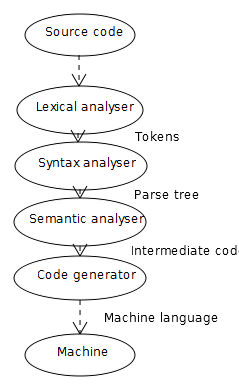
\includegraphics[scale=0.5]{pictures/compileroverview.png}
\capt{The different phases of a compiler. Based on Sebesta \textit{et al.}\cite{sebesta2013} p. 46, Figure 1.3}\label{fig:compileroverviewphases}
\end{figure}

\subsection{Lexical analysis}

Patterns of characters from alphabet -> tokens

\subsection{Syntax analysis}
All languages whether natural or artificial is a set of strings of characters over some alphabet. A language does not contain all possible strings over an alphabet. There are rules for how the strings can look that are in a language. Those rules can be specified formally to describe the syntax of a language\cite[p. 135]{sebesta2013}. A common way to describe a language's syntax is by a formal language-generation mechanism (also called grammars or context free grammars). By describing a grammar that can generate all possible strings in a language, the language has also been formally described. Backus-Naur Form is such a mechanism which in the 1950's became the most widely used method for describing programming language syntax\cite[p. 137]{sebesta2013}.

\begin{ebnf}
%Expressions
\grule{program}{\gter{print} expr}
\grule{expr}{\gter{(} \gcat term \gcat \gter{)} \gcat operator \gcat \gter{(} \gcat term \gcat \gter{)}}
\grule{operator}{\gter{=}}
\galt{\gter{>}}
\galt{\gter{<}}
\grule{term}{number}
\galt{expr}
\grule{number}{\textbf{any number}}
\end{ebnf}


\subsection{Semantic analysis}
\subsection{Code generation}
\subsection{Interpretation}

A pure interpretation of a program lies at the opposite end (from compilation) regarding to methods of implementation. With this approach, which can be see, on \figref{fig:compileroverviewinterpretation}, no translation is performed at all. An interpreter is interpreting a program written in the targeted language. It acts like a virtual machine which instructions are statements of high level language. By purely using interpretation, a source code debugger can easily be implemented. Various errors that might occur can once they are detected easily refer to which place in the source code that caused the error. The debugging is eased because the interpreter works like a software implementation of a virtual machine, thus the state of the machine and the value of a specific variable can be outputted at any time when requested. This will of course lead to the disadvantage that an interpreter uses more space than a compiler. Further more, the execution speed of an interpreter is usually 10 to 100 times slower than that of a compiler \cite[p. 48]{sebesta2013}.

\begin{figure}
\centering
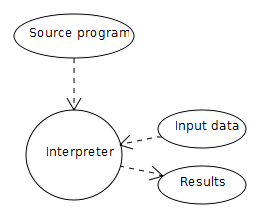
\includegraphics[scale=0.5]{pictures/compileroverviewinterpretation.png}
\capt{The different phases of an interpreter. Based on Sebesta \textit{et al.}\cite{sebesta2013} p. 48, Figure 1.4}\label{fig:compileroverviewinterpretation}
\end{figure}

The compiling or interpreting approach can be combined to form a hybrid implementation system. This method is illustrated in \figref{fig:compileroverviewhybrid}, where a program is compiled into an intermediate code which is then interpreted. By using this approach, errors in a program can be detected before interpretation which can save much time for a programmer. A great portability can also be achieved when using hybrid system. The initial implementation of Java was hybrid and allowed Java to be compiled to an intermediate code that could run on any platform which had an implementation of Java Virtual Machine\cite[p. 50]{sebesta2013}. 

\begin{figure}
\centering
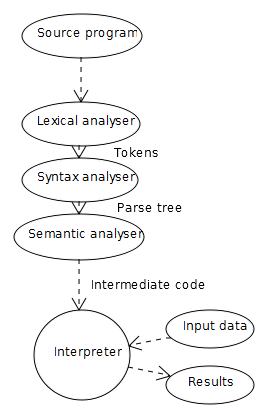
\includegraphics[scale=0.5]{pictures/compileroverviewhybrid.png}
\capt{The different phases of a hybrid implementation systems. Based on Sebesta \textit{et al.}\cite{sebesta2013} p. 49, Figure 1.5}\label{fig:compileroverviewhybrid}
\end{figure}